\chapter{DAWID, LLMs and Feature Detection}

We show the design and setup of the LLM AI interface and framework DAWID, integrating AI/ML based services, specific knowledge, functions and data with an LLM based chatbot interface. 

\begin{figure}[htbp]
    \centering
    \includegraphics[width=0.95\textwidth]{images/AI_Centre_Client_Server_Architecture.png}
    \caption{Client-server architecture for the AI Centre assistant system. The user interface connects to a backend server, which manages state, LLM calls, tool execution, and file storage. This structure enables interactive AI-driven workflows with persistent memory and modular tools.}
    \label{fig:ai-centre-architecture}
\end{figure}

%===============================================================================
%
%===============================================================================
\section{The DAWID Frontend: Upload and Interaction Interface}

The DAWID system provides a lightweight web interface for uploading data, sending user queries, and receiving processed responses. It is built using {\bf HTML} plus {\bf PHP}, styled with {\bf CSS}, and controlled by {\bf JavaScript} for asynchronous upload and interaction behavior.

%------------------------------------------------------------------------------
%
%------------------------------------------------------------------------------
\subsection*{Main Interface Structure}

The main page of the frontend is implemented in \texttt{index.php}, which includes the HTML layout for the upload and chat areas, links to the CSS style sheet and JavaScript functionality, and containers to display request and response output.

\begin{codeonly}{Excerpt from \texttt{index.php}}
<form id="uploadForm" method="post" enctype="multipart/form-data">
  <input type="file" id="uploadFile" name="uploaded_file">
  <div id="upload-result"></div>
</form>

<div id="request" class="query-heading">Waiting for request...</div>
<div id="response-container">
  <div id="response">Awaiting reply...</div>
</div>
\end{codeonly}

This HTML provides an upload form that will automatically submit when a file is selected. The response areas (`request`, `response`) are updated via JavaScript.

%------------------------------------------------------------------------------
%
%------------------------------------------------------------------------------
\subsection*{Asynchronous Upload: JavaScript Logic}

The file \texttt{dawid\_upload.js} automatically submits the form once a file is picked and uses the Fetch API to send it to the backend PHP script. The status messages are displayed in the frontend.

\begin{codeonly}{Automatic Upload via JavaScript}
fileInput.addEventListener("change", function() {
    if (fileInput.files.length) {
        uploadForm.requestSubmit();  // Auto-submit form
    }
});
\end{codeonly}

\begin{codeonly}{Submit Handler and Server Interaction}
uploadForm.addEventListener("submit", function (e) {
    e.preventDefault();
    const formData = new FormData();
    formData.append("uploaded_file", fileInput.files[0]);

    fetch("upload_handler.php", {
        method: "POST",
        body: formData,
    })
    .then(response => response.json())
    .then(data => {
        uploadResult.innerText = "Upload result: " + data.message;
    });
});
\end{codeonly}

%------------------------------------------------------------------------------
%
%------------------------------------------------------------------------------
\subsection*{Interactive JavaScript for Streaming and Sessions}

Beyond file uploads, DAWID's frontend JavaScript also enables live streaming of LLM responses and manages user interaction sessions. This enhances responsiveness and enables a smooth user experience with real-time feedback.

%------------------------------------------------------------------------------
%
%------------------------------------------------------------------------------
{\bf Streaming LLM Responses to the User.} The JavaScript in \texttt{display.js} handles streaming output from a backend Python process. It reads text chunks from the response as they arrive and updates the display accordingly.

\begin{codeonly}{Streaming Output Display Logic}
const responseDiv = document.getElementById("response");
const requestDiv = document.getElementById("request");

function streamResponse(url, body) {
    fetch(url, {
        method: "POST",
        headers: { "Content-Type": "application/json" },
        body: JSON.stringify(body)
    })
    .then(async response => {
        const reader = response.body.getReader();
        let partial = "";
        while (true) {
            const { done, value } = await reader.read();
            if (done) break;
            const chunk = new TextDecoder().decode(value);
            partial += chunk;
            responseDiv.innerHTML = marked.parse(partial);
        }
    });
}
\end{codeonly}

{\bf Streaming Display Logic.}
The \texttt{streamResponse} function implements real-time display of responses from a streaming LLM backend. It reads data chunks from the server using a \texttt{ReadableStream\-DefaultReader}, which is part of the Streams API built into modern web browsers, specifically part of the WHATWG Streams Standard. It appends each chunk to a growing \texttt{partial} string. 

After every chunk is received, the entire \texttt{partial} string is re-parsed using \texttt{marked.parse()} and set as the \texttt{innerHTML} of the output container. This ensures that the user sees an incrementally updated and fully formatted response as it arrives. Although this design re-parses the entire response repeatedly, it offers a simple and robust way to render streamed Markdown text progressively without missing updates or introducing formatting errors.


This creates a live feedback loop that immediately shows partial results as they are streamed from the server.

%------------------------------------------------------------------------------
%
%------------------------------------------------------------------------------
\subsubsection*{Session Control and Interaction History}

User inputs and responses are stored in a browser-local session using a chat-style layout. The history is updated dynamically with each turn. This is complementary to backend storage. 

\begin{codeonly}{Example: Appending Messages to the History}
function appendToHistory(role, content) {
	const block = document.createElement("div");
	block.className = role + "-message";
	block.innerHTML = marked.parse(content);
	responseContainer.appendChild(block);
}
\end{codeonly}

Each user message or system response is added as a new block, styled via CSS. This maintains continuity in the interaction and supports review or inspection by the user.

\vspace{1em}
Together, these JavaScript modules turn the DAWID frontend into a responsive, real-time interface for LLM-driven services, managing uploads, sessions, streaming results, and user-friendly interactions.

%------------------------------------------------------------------------------
%
%------------------------------------------------------------------------------
\subsection*{Styling the Interface}

The CSS file \texttt{dawid\_style.css} defines the visual structure of the containers, input elements, and the response area.

\begin{codeonly}{Styling Example: Upload and Response Blocks}
textarea, #response-container {
    width: 90%;
    max-width: 800px;
    box-sizing: border-box;
}

.container {
    width: 95%;
    background: white;
    padding: 20px;
    border-radius: 10px;
    box-shadow: 0px 0px 10px rgba(0, 0, 0, 0.1);
}
\end{codeonly}

These CSS classes ensure the DAWID interface is clean, centered, and readable across browsers.

%------------------------------------------------------------------------------
%
%------------------------------------------------------------------------------
\subsection*{Frontend Summary}

The DAWID frontend provides a responsive and extensible interface for interacting with AI-based backends. Its key features include:

\begin{itemize}
    \item \textbf{Intuitive file upload} with immediate user feedback using asynchronous JavaScript.
    \item \textbf{Streaming of LLM responses} using the Fetch API and a readable stream reader, enabling real-time display of partial outputs.
    \item \textbf{Session and history handling}, allowing each user to maintain a visible context of their interaction.
    \item \textbf{Dynamic Markdown rendering} of incoming content using \texttt{marked.js}, continuously updating the output with every chunk.
    \item \textbf{Modular design} that can be easily integrated with a backend handling LLM interaction and a wide range of specific functions in a flexible way with the LangChain, LangGraph, or other LLM orchestration frameworks.
\end{itemize}

This frontend architecture supports real-time interactions, enhances usability for AI-based assistants, and lays the groundwork for agent-driven web interfaces.

\begin{figure}[htbp]
    \centering
    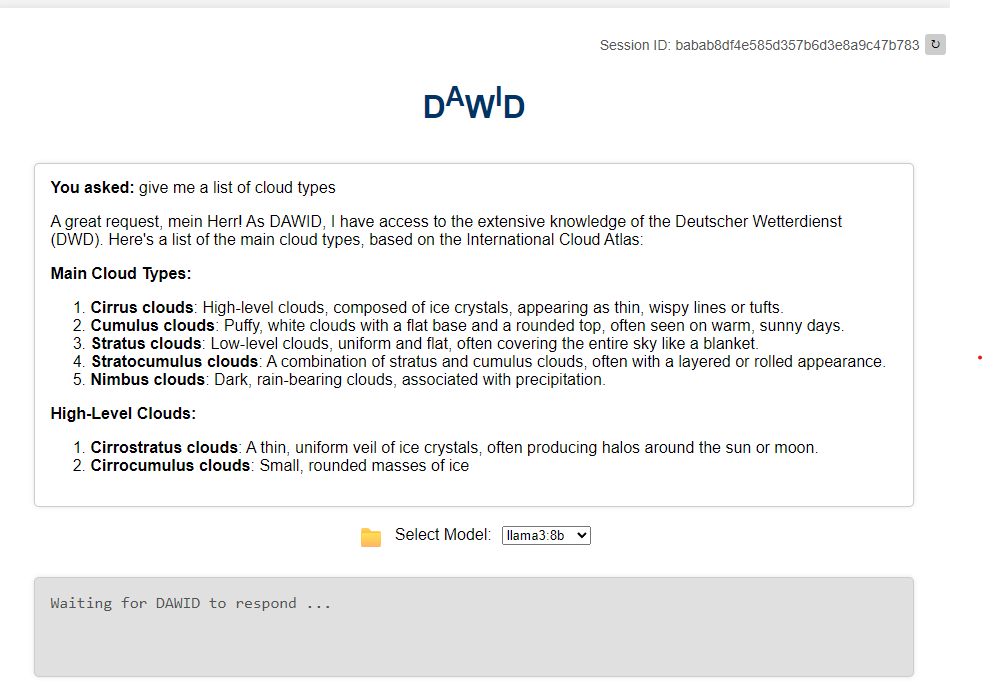
\includegraphics[width=0.95\textwidth]{images/dawid_interface1.png}
    \caption{Example DAWID frontend session: The assistant responds to a query on cloud types, listing categories based on the International Cloud Atlas. The reply is formatted using Markdown and streamed in real time.}
    \label{fig:dawid-cloudtypes}
\end{figure}

%===============================================================================
%
%===============================================================================
\section{DAWID Backend Architecture}

The DAWID backend is structured to provide a modular, extensible framework that connects a frontend assistant with powerful server-side components including local and remote language models, function execution, and LangGraph workflows.

%------------------------------------------------------------------------------
%
%------------------------------------------------------------------------------
\subsection*{Overview of Backend Components}

The backend consists of several Python modules that work together:
\begin{itemize}
    \item \texttt{dawid\_server.py}: Main entry point for API calls from the frontend. Manages request routing, user session IDs, and streaming responses.
    \item \texttt{dawid\_openai.py} and \texttt{dawid\_llama.py}: LLM wrappers for calling OpenAI or local \texttt{llama.cpp}-based models.
		\item \texttt{dawid\_users.py}: User management for accessing document spaces and functions. 
    \item \texttt{dawid\_functions.py}: Extracts structured function calls from LLM outputs (e.g., \texttt{get\_current\_weather}).
    \item \texttt{dawid\_graphs.py}: Defines and executes LangGraph graphs based on available functions and user goals.
\end{itemize}

This modular design enables easy extension: new functions can be added, new LLMs integrated, and complex agent workflows configured with LangGraph.

%------------------------------------------------------------------------------
%
%------------------------------------------------------------------------------
\subsection*{Session Handling and Routing}

Each interaction is assigned a unique \texttt{session\_id}. The server can distinguish multiple sessions, maintain short-term context, and route queries accordingly. This is crucial for multi-user operation and allows context-aware processing via LangGraph.

The main server logic is contained in \texttt{dawid\_server.py}, which accepts user queries via HTTP POST, determines the model to use, and invokes the appropriate backend logic.

%------------------------------------------------------------------------------
%
%------------------------------------------------------------------------------
\subsection*{User Management, Document Folders, and Context Retrieval / Retrieval Augmented Generation (RAG)}

DAWID implements a persistent user management system backed by an \texttt{SQLite} database. Each user is identified by a unique session or login ID and is associated with:

\begin{itemize}
    \item a private document folder (\texttt{docs/\{user\_id\}}),
    \item access to one or more group-shared folders (e.g., \texttt{docs/shared/\{group\_name\}}),
    \item a vector store (\texttt{faiss\_index}) built for each document folder.
\end{itemize}

This design allows both personalized and collaborative access to document content, enabling hybrid use cases such as private notes and shared projects.

When a user asks a question, the system performs a simple semantic analysis to decide whether document access is needed (e.g., for terms like \texttt{based on the uploaded file}, \texttt{summarize this report}, etc.), but also based on topics which are extracted from the document spaces and provided, such that topical search can trigger faiss retrieval and integration. If document access is inferred:

\begin{enumerate}
    \item A FAISS similarity search is triggered within the appropriate user or group folder.
    \item Relevant chunks are inserted into the LLM prompt as additional context.
    \item The response is generated with awareness of both conversation state and retrieved content.
\end{enumerate}

The document integration can be carried out based on a fast identification logic
as conceptually shown in the following code block. 

\begin{codeonly}{Topic-Aware Document Space Selection}
# Mapping from document space to list of covered topics (user-defined)
USER_SPACES = {
    "user/personal_notes": ["numerics", "python", "weather models"],
    "group/satellite_team": ["radiative transfer", "cloud detection", "satellite channels"],
    "group/forecasting": ["icon", "precipitation", "ensemble spread"]
}

# Determine which document spaces are relevant for the query
def topics_needed(query: str) -> list[str]:
    relevant_spaces = []

    for space, topics in USER_SPACES.items():
        for topic in topics:
            if topic in query.lower():
                relevant_spaces.append(space)
                break  # one hit is enough for this space

    return relevant_spaces

# Main document retrieval logic
def build_prompt_with_documents(query: str, user_id: str) -> str:
    if detect_intent_fast_llm(query) != "doc_query":
        return default_prompt(query)

    relevant_spaces = topics_needed(query)
    if not relevant_spaces:
        return default_prompt(query)

    # Retrieve context from each relevant FAISS index
    context_blocks = [
        faiss_retrieve(space, query) for space in relevant_spaces
    ]
    full_context = "\n\n".join(context_blocks)
    return build_prompt_with_context(query, full_context)
\end{codeonly}




%------------------------------------------------------------------------------
%
%------------------------------------------------------------------------------
\subsection*{LLM Abstraction and Streaming}

The modules \texttt{dawid\_openai.py} and \texttt{dawid\_llama.py} implement streaming query interfaces:

\begin{codeonly}{Streaming a Query via OpenAI}
def stream_openai_response(messages, model="gpt-4o-mini", temperature=0.2):
    ...
    for chunk in response:
        if chunk.choices[0].delta.content:
            yield chunk.choices[0].delta.content
\end{codeonly}

\begin{codeonly}{Streaming a Query via llama.cpp Server}
def stream_llama_response(messages, model="llama3"):
    ...
    async for chunk in response.aiter_lines():
        ...
        yield token
\end{codeonly}

This lets the frontend receive partial results in real-time — a major benefit for interactive user interfaces.

\textbf{Backend Language Model Infrastructure.} For in-house LLM inference, DAWID currently operates a set of \texttt{llama.cpp}-based servers deployed on high-performance, CPU-optimized machines. These servers host various models (e.g., \texttt{llama3:8b}) and are selected at runtime by the DAWID backend for parallel load distribution. While the current implementation uses random selection, this mechanism is being extended to a dynamic load balancer that considers real-time system load and response latency. This ensures efficient use of compute resources and consistent user experience under varying workloads.


%------------------------------------------------------------------------------
%
%------------------------------------------------------------------------------
\subsection*{Function Extraction and Graph Control}

After receiving a response from the LLM, \texttt{dawid\_functions.py} inspects the output for structured function calls. These are expected either as JSON blocks:

\begin{codeonly}{Example Function Call in JSON}
{
  "function_calls": [
    { "name": "get_current_datetime", "arguments": {} }
  ]
}
\end{codeonly}

If such a call is detected and valid (checked against \texttt{AVAILABLE\_FUNCTIONS}), the call is extracted and removed from the LLM output before further processing. 

%------------------------------------------------------------------------------
%
%------------------------------------------------------------------------------
\subsection*{LangGraph Execution}

The LangGraph graph is built and run using the function \texttt{create\_dawid\_graph()} in \texttt{dawid\_graphs.py}.

\begin{itemize}
    \item The graph starts with \texttt{get\_current\_datetime}.
    \item It branches based on whether a weather function is also requested.
    \item Each node modifies the shared state dictionary.
\end{itemize}

\begin{codeonly}{Creating a LangGraph Flow}
graph.add_node("get_current_datetime", get_current_datetime_node)
graph.add_conditional_edges("get_current_datetime", branch_logic, {
    "get_current_weather": "get_current_weather",
    "end": END
})
\end{codeonly}

%------------------------------------------------------------------------------
%
%------------------------------------------------------------------------------
\subsection*{Extensible DAWID System}

New tools, such as plotting, file downloads, or model-based simulation, can be added as functions. To do so:
\begin{enumerate}
    \item Add the function name to \texttt{AVAILABLE\_FUNCTIONS} in \texttt{dawid\_functions.py}.
    \item Implement the function node in \texttt{dawid\_graphs.py}.
    \item Extend the branching logic if needed.
\end{enumerate}

This architecture allows DAWID to act as a semi-autonomous assistant with tool access, language model integration, and structured workflows, integrated with specific knowledge which can be made available to users by adding them to document spaces. 

%------------------------------------------------------------------------------
%
%------------------------------------------------------------------------------
\subsection*{Privacy and Data Security}
The DAWID backend is hosted entirely on internal DWD infrastructure and protected by a dedicated firewall, ensuring that user interactions and uploaded data remain strictly within the organization's secure network. User-specific data, including session history, uploaded files, and document-based context, is stored in user- and group-specific folders, isolated from external access.

Additionally, the in-house deployment of the llama3:8b language model ensures that queries processed via this model never leave the building. This enables secure, high-quality local inference with full data confidentiality — ideal for sensitive or internal-use cases.

\vspace{0.5em}
\textbf{Further security and privacy features:}
\begin{itemize}
\item \textbf{FAISS vector search is local.} Any retrieval-augmented generation (RAG) or document search operations are carried out via local FAISS indices, which never transmit queries or data externally.
\item \textbf{Session-based data control.} Each session is tied to a unique ID and limited in scope, allowing for controlled cleanup or persistence according to policy.
\item \textbf{Optional OpenAI integration.} If the user selects an OpenAI model, the request is processed via the user’s OpenAI Platform account and subject to OpenAI’s privacy policy. The frontend allows full transparency and control over the selected model.
\item \textbf{Logging and audit trails.} Interactions can optionally be logged locally for auditing, debugging, or research under strict access controls.
\item \textbf{Future addition:} Fine-grained access rights to group folders and shared knowledge bases are implemented, with access through the DAWID user management.
\end{itemize}

This hybrid approach ensures that users benefit from local, private computation where needed while retaining the flexibility to use cloud-based services when desired.

\textbf{Infrastructure and Secure Communication.} The DAWID frontend is hosted on a professional-grade web server with a trusted TLS certificate, ensuring encrypted communication between users and the platform. Access to the backend services is tightly controlled: only the authorized Python process running on the frontend server is permitted to communicate with the DAWID server’s API port through an internal firewall. This isolation prevents unauthorized external access and ensures a secure and trusted environment for all interactions.


%===============================================================================
%
%===============================================================================
\section{AI based Feature Detection for Fronts}

This section describes a deep learning system for detecting weather fronts from meteorological input fields. The system includes both training and inference components and is designed to identify synoptic-scale structures based on surface-level atmospheric data. The approach leverages convolutional neural networks and standard PyTorch utilities, and is fully implemented in a modular set of Jupyter notebooks.

%------------------------------------------------------------------------------
\subsection{Overview and Objective}

Fronts are transition zones between air masses with distinct temperature and humidity characteristics. Detecting them automatically from gridded analysis or forecast data is a challenging task due to their complex structure and temporal evolution.

The AI front detection system uses supervised learning to train a model on labeled frontal maps. The trained model is then applied to both analysis and forecast fields to detect fronts in operational-style datasets.

%------------------------------------------------------------------------------
\subsection{Data and Preprocessing}

The input data for the front detection model consists of six meteorological fields extracted from numerical weather prediction model outputs (ICON GRIB files) on a regular latitude-longitude grid with approximately 0.4° horizontal resolution. The selected fields are:

\begin{itemize}
  \item {\bf PMSL}: Mean sea-level pressure (\texttt{shortName = prmsl})
  \item {\bf T2M}: 2-meter temperature (\texttt{shortName = t2m})
  \item {\bf RH2M}: 2-meter relative humidity (\texttt{shortName = r2})
  \item {\bf U10M}: 10-meter zonal wind component (\texttt{shortName = u10})
  \item {\bf V10M}: 10-meter meridional wind component (\texttt{shortName = v10})
  \item {\bf FRLAND}: Land-sea mask (binary 1/–1 from external GRIB file)
\end{itemize}

Each field is normalized channel-wise to a comparable numerical range in order to stabilize training. The normalization constants are determined from a large set of training data statistics:

\begin{codeonly}{Input Normalization}
PMSL = (PMSL - 101280.7) / 1145.4
T2M  = (T2M  - 277.2)    / 14.2
RH2M = (RH2M - 79.0)     / 14.1
U10M = (U10M - 0.8)      / 5.1
V10M = (V10M - (-0.1))   / 5.2
FRLAND[FRLAND > 0] = 1
FRLAND[FRLAND == 0] = -1
ICON = np.stack([PMSL, T2M, RH2M, U10M, V10M, FRLAND], axis=0)
\end{codeonly}

The resulting array has shape \texttt{[6, lat, lon]} and is stored in NetCDF files with dimensions \texttt{var}, \texttt{lat}, and \texttt{lon}. Each file corresponds to one analysis or forecast time step.

The corresponding labels used for supervised training are categorical 2D frontal maps, where each grid point belongs to one of several classes: background (no front), warm front, cold front, or occluded front. These labels are used in combination with a multi-class cross-entropy loss during model training.



%------------------------------------------------------------------------------
\subsection{Model Architecture}

The front detection model is a U-Net architecture, a popular design for semantic segmentation tasks. It consists of a contracting path that extracts multi-scale features through convolutions and a symmetric expanding path that enables precise localization by combining upsampled features with high-resolution activations from earlier layers.

In this application, the U-Net accepts 6 input channels and outputs a 4-channel segmentation map, corresponding to different frontal types or background.

\begin{codeonly}{Model Architecture}
# Load model from external repository or local file
model = unet.UNet(in_channels=6, out_channels=4, init_features=64)
model = model.to(device)
\end{codeonly}

The model is optimized using the AdamW optimizer and categorical loss:

\begin{codeonly}{Loss and Optimizer}
loss_fn   = nn.CrossEntropyLoss().to(device)
optimizer = torch.optim.AdamW(params=model.parameters(), lr=0.0001)
\end{codeonly}

This architecture enables high-resolution frontal feature detection by preserving spatial detail through skip connections and deep supervision.


%------------------------------------------------------------------------------
\subsection{Training Procedure}

Training is handled by the notebook \texttt{aifronts\_torch\_training.ipynb}. The model is trained using categorical cross-entropy loss over multi-class front maps, with classes typically corresponding to warm, cold, occluded fronts, and background. 

The training loop includes early stopping based on validation loss, online evaluation, and MLflow-based logging. Accuracy is computed per epoch using a helper function that compares predicted classes with true labels.

Before training, model weights can optionally be restored from a previous checkpoint:

\begin{codeonly}{Optional Retraining}
retrain = False
if retrain:
    print("Loading existing model weights")
    model.load_state_dict(torch.load("best-model-parameters.pt"))
\end{codeonly}

Early stopping is controlled by a fixed patience and maximum number of epochs:

\begin{codeonly}{Training Parameters}
best_avg_vloss = 1000  # Initial high value
stp            = 0     # Early stopping counter
stopafter      = 5     # Stop if no improvement after N epochs
max_epochs     = 200
\end{codeonly}

The MLflow experiment is initialized before training begins. To avoid issues with DWD-internal proxies, proxy variables are explicitly removed from the environment:

\begin{codeonly}{MLflow Setup}
for key in ("HTTP_PROXY","http_proxy","HTTPS_PROXY","https_proxy"):
    if key in os.environ:
        del os.environ[key]

os.environ['MLFLOW_TRACKING_USERNAME'] = 'ffundel'
os.environ['MLFLOW_TRACKING_PASSWORD'] = 'mlflowffundel'
mlflow.end_run()
mlflow.set_tracking_uri("http://172.16.112.218:5051")
mlflow.set_experiment("aifronts_torch_felix")
mlflow.autolog()
run_name = datetime.today().strftime('%Y%m%d%H%M%S')
mlflow.start_run(run_name="unet-" + run_name)
\end{codeonly}

The training loop proceeds epoch-wise, alternating between training and validation mode:

\begin{codeonly}{Epoch Loop}
for epoch in range(max_epochs):
    model.train()
    for inputs, labels in train_loader:
        inputs, labels = inputs.to(device), labels.to(device)
        optimizer.zero_grad()
        outputs = model(inputs)
        loss = loss_fn(outputs, labels)
        acc  = accuracy(outputs, labels)
        loss.backward()
        optimizer.step()
\end{codeonly}

After training, validation metrics are calculated without gradient tracking:

\begin{codeonly}{Validation Loop}
    model.eval()
    with torch.no_grad():
        for vinputs, vlabels in validation_loader:
            vinputs, vlabels = vinputs.to(device), vlabels.to(device)
            voutputs = model(vinputs)
            vloss    = loss_fn(voutputs, vlabels)
            vacc     = accuracy(voutputs, vlabels)
\end{codeonly}

Training and validation metrics are recorded to the MLflow server after each epoch:

\begin{codeonly}{Metric Logging and Checkpointing}
    mlflow.log_metric("train_loss",     avg_loss,  step=epoch)
    mlflow.log_metric("train_accuracy", avg_acc,   step=epoch)
    mlflow.log_metric("eval_loss",      avg_vloss, step=epoch)
    mlflow.log_metric("eval_accuracy",  avg_vacc,  step=epoch)

    if avg_vloss < best_avg_vloss:
        stp = 0
        best_avg_vloss = avg_vloss
        print("Saving current model")
        torch.save(model.state_dict(), "best-model-parameters.pt")
    else:
        stp += 1

    if stp >= stopafter:
        break
\end{codeonly}

This loop ensures that only the best-performing model (based on validation loss) is retained and that each run is reproducibly logged and tracked. The combination of early stopping, metric logging, and weight checkpointing ensures both efficiency and traceability.



\begin{figure}[ht]
  \centering
  \begin{tabular}{ccc}
    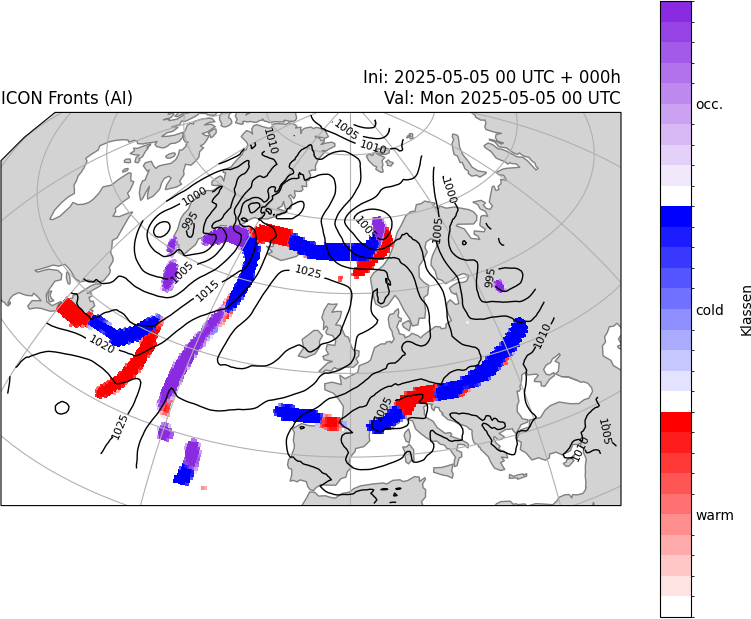
\includegraphics[width=0.3\textwidth]{images/plot_000.png} &
    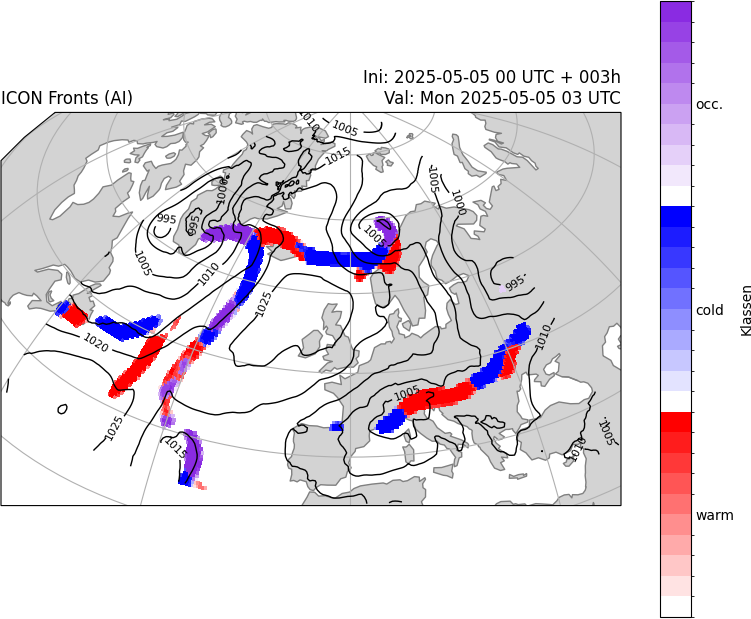
\includegraphics[width=0.3\textwidth]{images/plot_001.png} &
    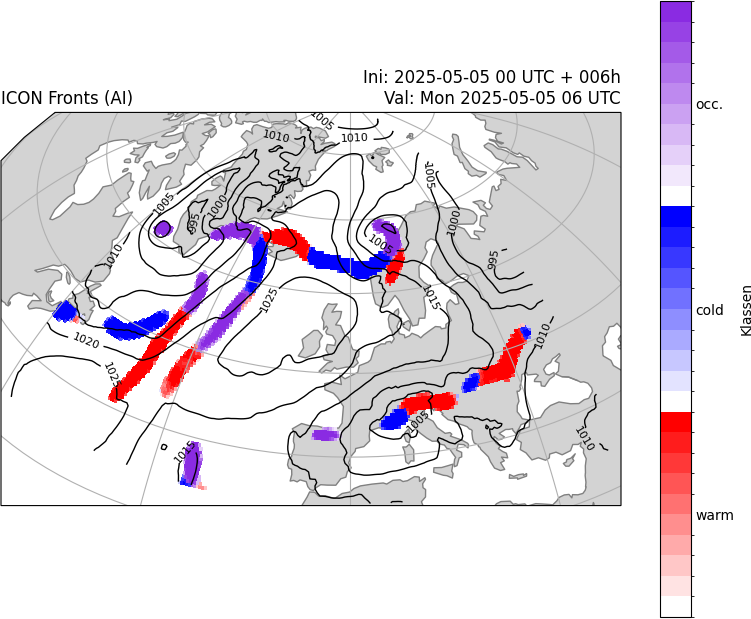
\includegraphics[width=0.3\textwidth]{images/plot_002.png} \\
    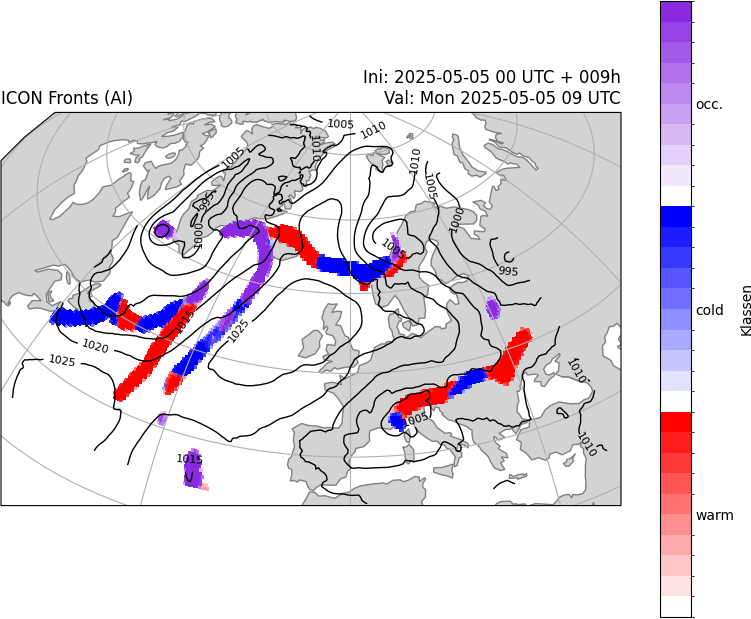
\includegraphics[width=0.3\textwidth]{images/plot_003.png} &
    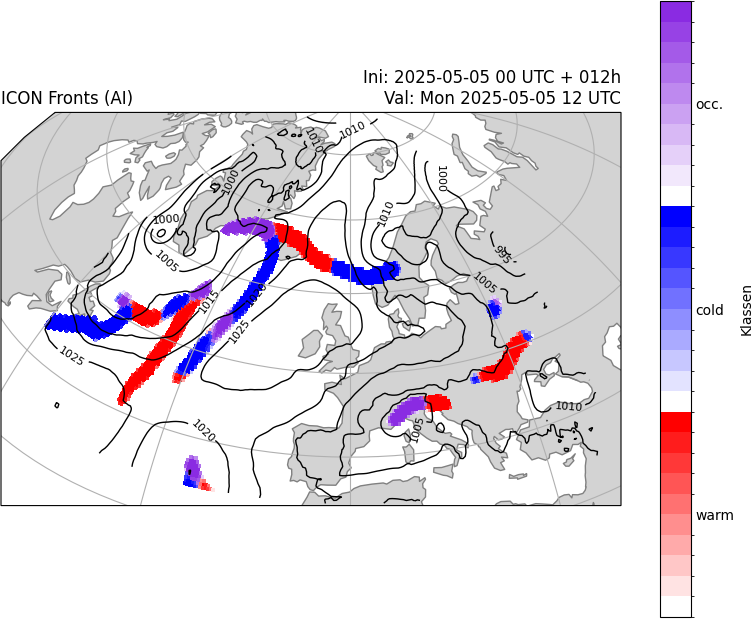
\includegraphics[width=0.3\textwidth]{images/plot_004.png} &
    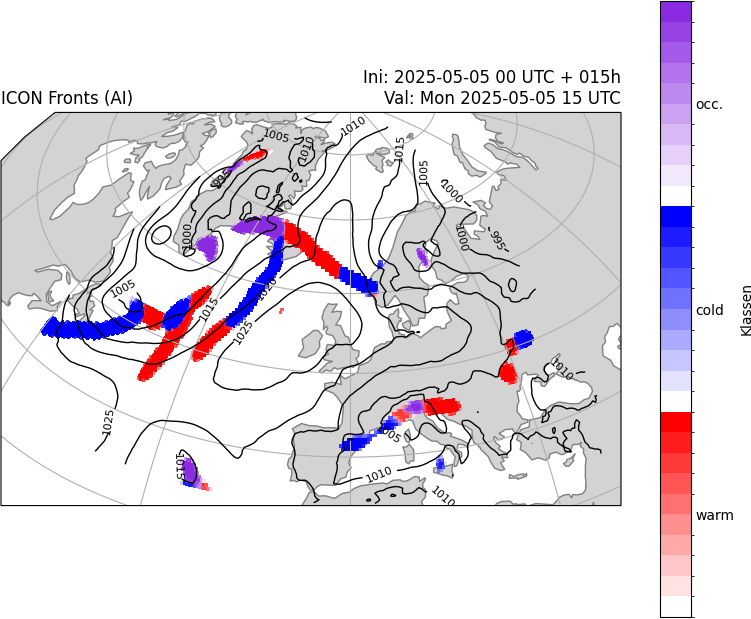
\includegraphics[width=0.3\textwidth]{images/plot_005.png} \\
  \end{tabular}
  \caption{Detected fronts from the AI model applied to ICON forecast fields initialized on 5 May 2025 at 00 UTC. Each map shows one forecast lead time (from +00h to +15h in 3h steps). The color-coded front detections correspond to warm fronts (red), cold fronts (blue), and occluded fronts (purple). Overlaid black contours show the corresponding mean sea-level pressure (MSLP), helping to interpret the synoptic environment. The AI system provides consistent front structures that evolve smoothly over time, following cyclonic systems and frontal zones in the pressure field.}
  \label{fig:forecast_fronts}
\end{figure}


%------------------------------------------------------------------------------
\subsection{Inference and Forecast Application}

Inference is handled in the notebook \texttt{aifronts\_torch\_inference.ipynb}, which loads the trained U-Net model and applies it to an ICON forecast field sequence. Input fields are already normalized and stored as NetCDF files with shape \texttt{[6, lat, lon]}. These are loaded and concatenated over time using \texttt{xarray}.

\begin{codeonly}{Load Normalized Forecast Input}
FCPATH      = "/.../input/"
DATE        = "2025050500"
FILES       = sorted(glob.glob(FCPATH + DATE + '/*.nc'))
datasets    = [xr.open_dataset(f) for f in FILES]
combined_ds = xr.concat(datasets, dim='time')
Input       = torch.tensor(combined_ds['ICON'].values, dtype=torch.float)
\end{codeonly}

The trained model is loaded and put into inference mode. It is then applied to the entire forecast sequence in one batch:

\begin{codeonly}{Run Inference}
best_model = UNet(in_channels=6, out_channels=4, init_features=30)
best_model.load_state_dict(torch.load("best-model-parameters.pt"))
best_model.eval()
inference  = best_model(Input)
\end{codeonly}

The model output is a 4-class probability map for each forecast time and grid point. This is postprocessed into a discrete field using \texttt{argmax} logic, with a special handling for the background (class 3):

\begin{codeonly}{Postprocessing to Class Index}
fc          = np.array(inference.detach().numpy())
fc[:,3,:,:] = np.where(fc[:,3,:,:] > 0.95, fc[:,3,:,:], np.nan)
fc          = np.nanargmax(fc, axis=1)
fc          = np.where(fc == 3, np.nan, fc)
fc[fc == 0] = inference.detach().numpy()[:,0,:,:][fc == 0]
fc[fc == 1] = inference.detach().numpy()[:,1,:,:][fc == 1] + 1
fc[fc == 2] = inference.detach().numpy()[:,2,:,:][fc == 2] + 2
\end{codeonly}

The resulting class predictions are combined with the original input MSLP field to create a joint array for visualization:

\begin{codeonly}{Create Output DataArray}
coords = {'type': ['fc', 'ps'],
          'case': range(57),
          'lat': combined_ds['lat'].values,
          'lon': combined_ds['lon'].values}
arr = xr.DataArray([fc, combined_ds["ICON"].values[:,0,:,:]], coords)
\end{codeonly}

A plot loop then visualizes each lead time of the forecast. The predicted fronts are shown as colored maps overlaid with MSLP contours and geographic context using Cartopy:

\begin{codeonly}{Plot Forecast Fronts}
for case in range(arr.shape[1]):
    dt = datetime.strptime(os.path.basename(os.path.dirname(FILES[case])), '%Y%m%d%H')
    vt = dt + timedelta(hours=case*3)

    data         = arr[0, case, :, :]
    contour_data = (arr[1, case, :, :] * 11.454) + 1012.807  # inverse normalization

    # Cartopy projection and layers
    fig = plt.figure(figsize=(10, 8))
    ax = plt.axes(projection=ccrs.Orthographic(0, 35))
    ax.add_feature(cfeature.NaturalEarthFeature('physical', 'land', '110m', facecolor='lightgray'), zorder=0)
    ax.coastlines(zorder=0, color='gray')
    ax.gridlines()

    # Color mapping for front types
    custom_cmap = build_custom_cmap()  # red = warm, blue = cold, violet = occluded
    bounds = np.linspace(0, 3, 31)
    norm = mcolors.BoundaryNorm(bounds, custom_cmap.N)

    # Plot fronts and MSLP
    mesh = ax.pcolormesh(Lon, Lat, data, cmap=custom_cmap, norm=norm, transform=ccrs.PlateCarree())
    contour_lines = ax.contour(Lon, Lat, contour_data, levels=np.arange(900, 1100, 5),
                               colors='black', linewidths=1, transform=ccrs.PlateCarree(), zorder=3)
    ax.clabel(contour_lines, inline=True, fontsize=8)

    # Titles and save
    ax.set_title("Ini: " + dt.strftime('%Y-%m-%d %H UTC') + " + " + str(case*3).zfill(3) + "h", loc="right")
    plt.title("ICON Fronts (AI)", loc="left")
    plt.savefig(f"plots/plot_{str(case).zfill(3)}.png")
    plt.close(fig)
\end{codeonly}

This inference process is repeated over the entire forecast time range (e.g., 57 time steps). The resulting maps as displayed in Figure \ref{fig:forecast_fronts} illustrate the temporal evolution of predicted front positions and their meteorological environment, enabling visual inspection or further automated verification.



